\section{Comparision}\label{Sec:Com}
\subsection{Backpack}
The \texttt{backpack small8.fld} file contains the volume of a backpack with its content. 
Volume rendering could be useful to display the content of the volume without looking in to the bag.
This is already done at the airport with different techniques.
The idea is to find dangerous items in the bag. 
So scanning the volume is useful when we can see the content of the bag. 
\begin{figure}[H]
	\centering
	\begin{subfigure}[t]{0.45\textwidth}
		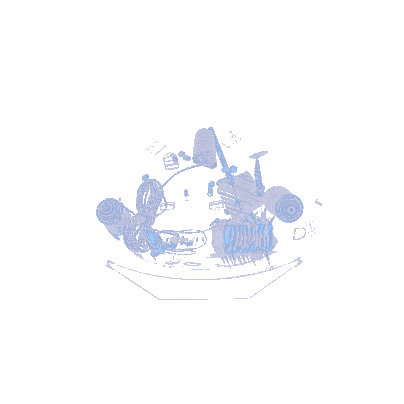
\includegraphics[width=\textwidth]{fig_comp_bp_first60}
		\caption{Rendered using the first method with first on 60}
	\end{subfigure}
	~%
	\begin{subfigure}[t]{0.45\textwidth}
		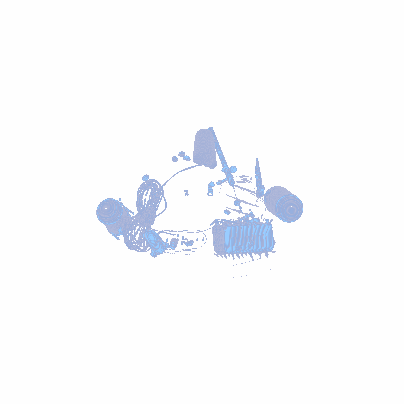
\includegraphics[width=\textwidth]{fig_comp_bp_first100}
		\caption{Rendered using the first method with first on 100}
	\end{subfigure}
	
	\begin{subfigure}[t]{0.45\textwidth}
		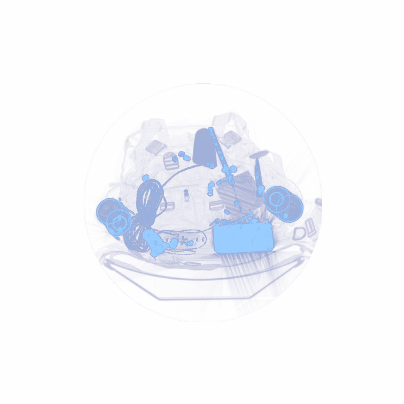
\includegraphics[width=\textwidth]{fig_comp_bp_mip}
		\caption{Rendered using the maximum intensity projection}
	\end{subfigure}
	~%
	\begin{subfigure}[t]{0.45\textwidth}
		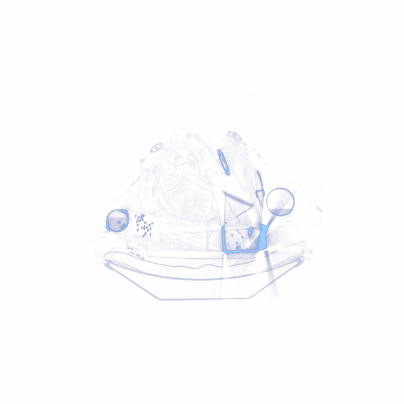
\includegraphics[width=\textwidth]{fig_comp_bp_slicer}
		\caption{Rendered using the already implemented slicer method}
	\end{subfigure}
	\caption{A comparison of rendering \texttt{backpack small8.fld} with different rendering methods}
	\label{fig:comp:bp}
\end{figure}
	
\begin{figure}[H]
	\ContinuedFloat
	\centering
	\begin{subfigure}[t]{0.45\textwidth}
		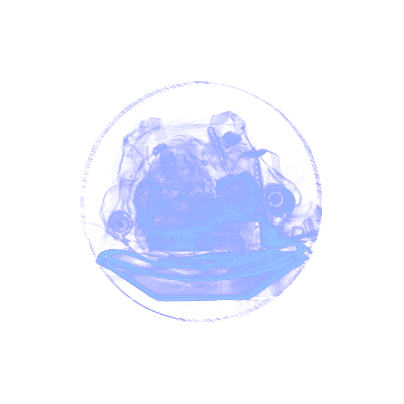
\includegraphics[width=\textwidth]{fig_comp_bp_ctfftb}
		\caption{Rendered using the composite transfer function Front to Back}
	\end{subfigure}
	~%
	\begin{subfigure}[t]{0.45\textwidth}
		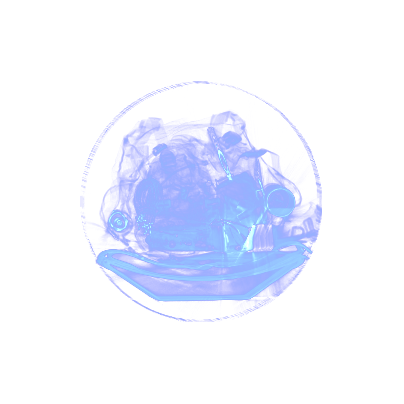
\includegraphics[width=\textwidth]{fig_comp_bp_ctfbtf}
		\caption{Rendered using the composite transfer function Back to Front}
	\end{subfigure}
	
	\caption{A comparison of rendering \texttt{backpack small8.fld} with different rendering methods}
	\label{fig:comp:bp}
\end{figure}
When we look at the images in \ref{fig:comp:bp}, we can see that some techinques excel at this and others do not. 
We will first discuss which techniques are not really useful. 
The slicer and composite transfer functions do not show all content of the bag.
The both first do not display everything nicely, but the maximum intensity projection shows the  most useful content of the bag. 
So we think that maximum intensity projection would be the best choice with the standard transfer function.
However we can adjust the transfer function to make the composite transfer function more useful.
As you can see in \ref{fig:comp:backpak} we can also use the composite transfer function for this.
\begin{figure}[H]
	\centering
		
\includegraphics[width=0.45\textwidth]{backpack}
		\caption{Rendered backpack with the composite transfer function with a custom transfer function}
	\label{fig:comp:backpak}
\end{figure}
\subsection{Pig}
The \texttt{pigl8.fld} file contains the volume of a pig money-box with some coins in it.
Volume rendering could be useful to display to know how much money is in the pig.
At first we thought this could be done best with the maximum intensity projection.
As you can see in \ref{fig:comp:big}, the intensity of the coins is lower than that of the outside. 
This means we cannot use the maximum intensity projection to count the coins. 
Also the first method and the composite transfer fuction front to back do not show any coins. 
The two methods that show the coins are the slicer and the composite transfer function back to front. 
The slicer could miss some coints, but is easier to count. 
The back to front method is more likely to show all coins, but might be harder to count when there are more coins. 
\begin{figure}[H]
	\centering
	\begin{subfigure}[t]{0.45\textwidth}
		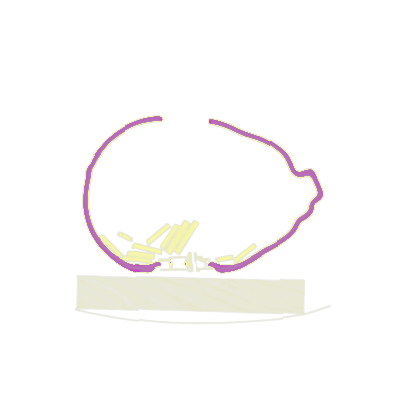
\includegraphics[width=\textwidth]{fig_comp_big_slicer}
		\caption{Rendered using the already implemented slicer method}
	\end{subfigure}
	~%
	\begin{subfigure}[t]{0.45\textwidth}
		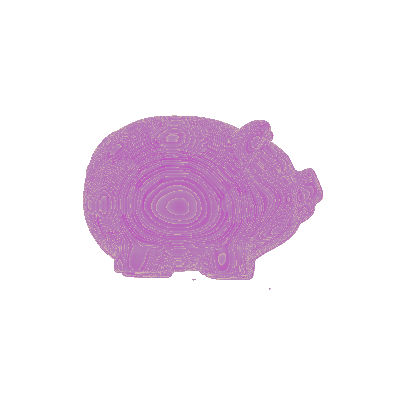
\includegraphics[width=\textwidth]{fig_comp_big_first108}
		\caption{Rendered using the first method with first on 108}
	\end{subfigure}
	
	\begin{subfigure}[t]{0.45\textwidth}
		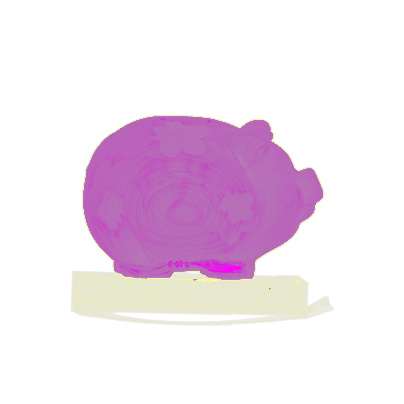
\includegraphics[width=\textwidth]{fig_comp_big_mip}
		\caption{Rendered using the maximum intensity projection}
	\end{subfigure}
	~%
	\begin{subfigure}[t]{0.45\textwidth}
		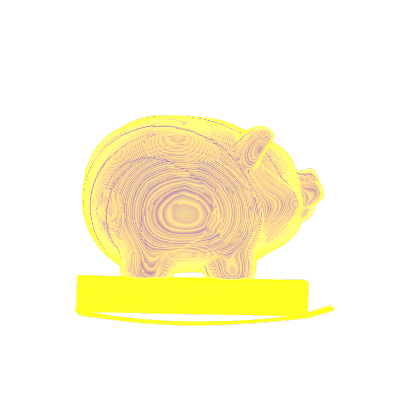
\includegraphics[width=\textwidth]{fig_comp_big_ctfftb}
		\caption{Rendered using the composite transfer function Front to Back}
	\end{subfigure}
	\caption{A comparison of rendering \texttt{big8.fld} with different rendering methods}
	\label{fig:comp:big}
\end{figure}
	
\begin{figure}[H]
	\ContinuedFloat
	\centering
	\begin{subfigure}[t]{0.45\textwidth}
		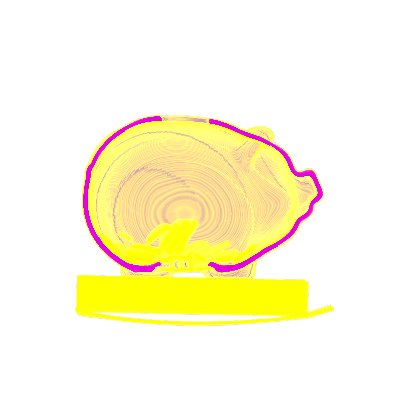
\includegraphics[width=\textwidth]{fig_comp_big_ctfbtf}
		\caption{Rendered using the composite transfer function Back to Front}
	\end{subfigure}
	~%
	\begin{subfigure}[t]{0.45\textwidth}
		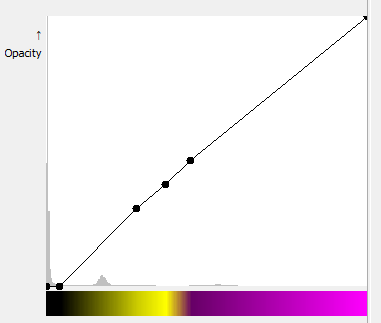
\includegraphics[width=\textwidth]{fig_comp_big_TF}
		\caption{The transfer function we used for rendering the images}
	\end{subfigure}
	
	\caption{A comparison of rendering \texttt{big8.fld} with different rendering methods}
	\label{fig:comp:big}
\end{figure}	
However we can adjust the transfer function to make the composite transfer function more useful.
As you can see in \ref{fig:comp:biggie} we can make the coins better visible.
\begin{figure}[H]
	\centering
		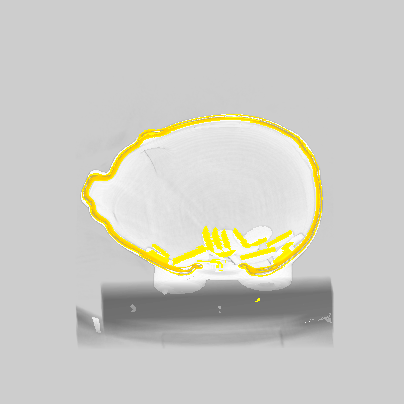
\includegraphics[width=0.45\textwidth]{pig}
		\caption{Rendered big with the composite transfer function with a custom transfer function}
	\label{fig:comp:biggie}
\end{figure}
\subsection{Gradient-based opacity weighting}
Using the gradient-based opacity weighting settings and the export function of our application, we created an animated GIF of the \texttt{carp8.fld} data set.
By rendering at different settings (increasing the $f_{min}$ parameter), we were able to first hide all the soft flesh of the fish until only the bone remains.
If we increase the minimum required density even more, we see that the smaller and softer bones start to disappear, until finally, the entire fish is gone.

The rendered GIF file is included with this report (since the bones are rendered in white, it is recommended to watch this with a dark background), but it is also hosted online at \url{http://imgur.com/zRD7NEw}.
Figure~\ref{fig:comp:carp} shows some frames of the animation.

All renders were created with these constants: $f_{max}$ of 240, $o_{min}$ of $0.6$ and $o_{max}$ of $0.8$.

\begin{figure}[H]
	\centering
	\begin{subfigure}[t]{0.45\textwidth}
		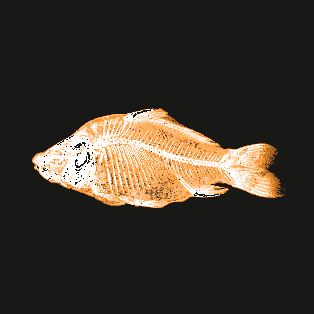
\includegraphics[width=\textwidth]{vis-010}
		\caption{$f_{min}$ of 70}
	\end{subfigure}
	~%
	\begin{subfigure}[t]{0.45\textwidth}
		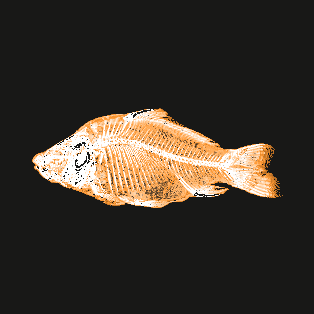
\includegraphics[width=\textwidth]{vis-040}
		\caption{$f_{min}$ of 100}
	\end{subfigure}
	
	\begin{subfigure}[t]{0.45\textwidth}
		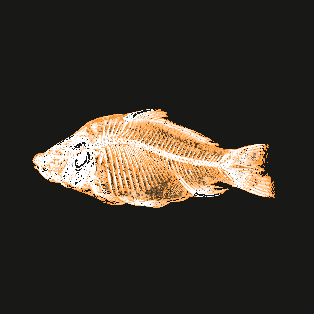
\includegraphics[width=\textwidth]{vis-080}
		\caption{$f_{min}$ of 140}
	\end{subfigure}
	~%
	\begin{subfigure}[t]{0.45\textwidth}
		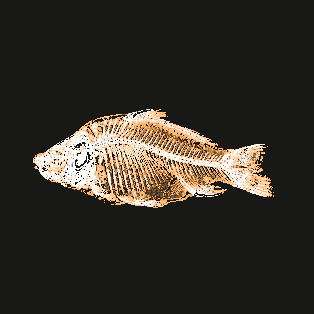
\includegraphics[width=\textwidth]{vis-100}
		\caption{$f_{min}$ of 160}
	\end{subfigure}
	\caption{A comparison of rendering \texttt{carp8.fld} at different gradient-based opacity weighing settings}
	\label{fig:comp:big}
\end{figure}
	
\begin{figure}[H]
	\ContinuedFloat
	\centering
	\begin{subfigure}[t]{0.45\textwidth}
		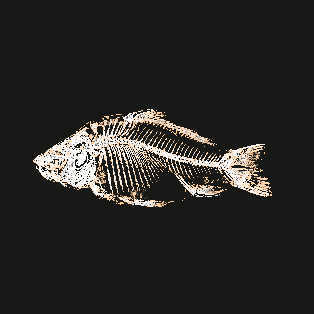
\includegraphics[width=\textwidth]{vis-115}
		\caption{$f_{min}$ of 175}
	\end{subfigure}
	~%
	\begin{subfigure}[t]{0.45\textwidth}
		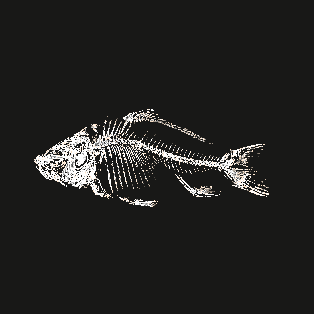
\includegraphics[width=\textwidth]{vis-130}
		\caption{$f_{min}$ of 190}
	\end{subfigure}
	
	\begin{subfigure}[t]{0.45\textwidth}
		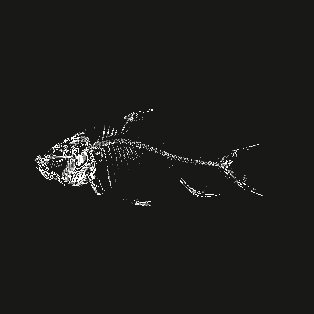
\includegraphics[width=\textwidth]{vis-150}
		\caption{$f_{min}$ of 210}
	\end{subfigure}
	~%
	\begin{subfigure}[t]{0.45\textwidth}
		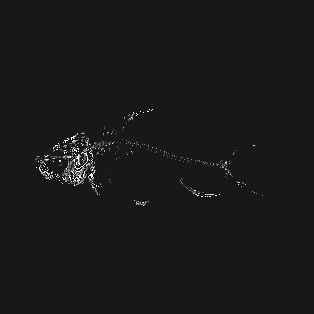
\includegraphics[width=\textwidth]{vis-160}
		\caption{$f_{min}$ of 220}
	\end{subfigure}
	
	\caption{A comparison of rendering \texttt{carp8.fld} at different gradient-based opacity weighing settings}
	\label{fig:comp:big}
\end{figure}
